\section*{Results}

We simulated \SI{5e5} synapses evolving as Kesten processes and recorded lifetime and weight distributions. For unbiased additive change ($\mu_b =0$), a power law like distribution of synaptic lifetimes emerges (Fig.~\ref{fig:lifetimes}A). The distribution of spine sizes $X_{T_{\text{max}}}$ resembles a log-normal distribution, as one might expect from findings on the synaptic weight distributions in cortical circuits \cite{Song2005}.

\vspace{1.2cm}
\begin{overpic}[width=\columnwidth]%
  % 110, 133
  {figures/lifetimes_weights.pdf}
  %\put(32,\ylin){anisotropic}
  \put(1,28){\normalfont \textbf{A}}
  \put(52,28){\normalfont \textbf{B}}
\end{overpic}
\captionof{figure}[format=hang,indention=1cm]{Dynamical properties of network connectivity modelled by Kesten processes. \textbf{A} Lifetime distribution of synapses created at time step $T_{\text{init}}$ uniformly distributed in $[0, T_{\text{max}}]$. \textbf{B} Distribution of spine sizes $X_{T_{\text{max}}}$ at time step $X_{T_{\text{max}}}$ (grey) and log-normal fit (red). Parameters for both: $a=0.9987$, $\mu_b=0$, $\sigma_b^2=0.22$, $X_{\text{insert}}=0.1$, $X_{\text{prune}}=0.01$. \label{fig:lifetimes}}

\vspace{3cm}

%% \begin{center}\vspace{1cm}
%%   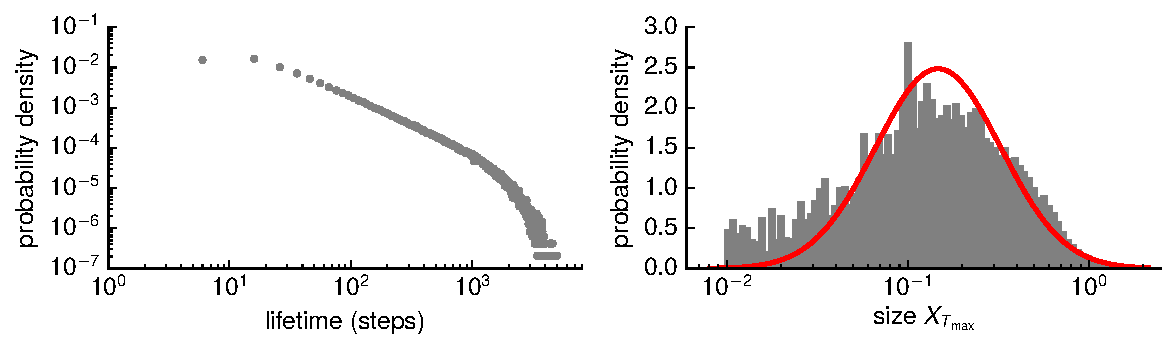
\includegraphics[width=\columnwidth]{%
%%     %% /home/fh/sci/lab/syn_lt/kesten_model/note_x/km_ca_rts_dd/img/lifetimes_weights.png}
%%     figures/lifetimes_weights.png}

%%   \captionof{figure}{}
%%   \label{fig:lifetimes}
%% \end{center}\vspace{1cm}

Next, we explored how different parameters in the model affect the lifetime and spine size distributions. We found that varying $\sigma_b^2$ has little effect on the distributions. Interestingly however, the bias in the additive change affects both distributions significantly. As one might expect, a bias towards increases in size moves the tail of the lifetime distribution towards higher lifetimes (Fig.~\ref{fig:lifemub}A) while shifting the mean of the spine size towards higher values (Fig.~\ref{fig:lifemub}B). This observation matches qualitatively with preliminary results from detailed network simulations in which a higher bias towards LTP resulted in similarly extended lifetimes.

  \vspace{1.4cm}
\begin{overpic}[width=\columnwidth]%
  % 110, 133
  {figures/lifetimes_weights_mub_compare.pdf}
  %\put(32,\ylin){anisotropic}
  \put(1,28){\normalfont \textbf{A}}
  \put(52,28){\normalfont \textbf{B}}
\end{overpic}
  \captionof{figure}{The bias of additive change in size strongly affects both lifetime and weight distributions. \label{fig:lifemub}}

  \vspace{1.8cm}
